\documentclass[a4paper,titlepage]{article}
\usepackage{graphicx}
\usepackage{subcaption}
\usepackage[default,oldstyle,scale=0.95]{opensans} %% Alternatively
%% use the option 'defaultsans' instead of 'default' to replace the
%% sans serif font only.
\usepackage[margin=1in]{geometry}
\usepackage[table]{xcolor}
\usepackage{awesomebox}
\usepackage{tcolorbox}

\usepackage[T1]{fontenc}
\usepackage{setspace}
\usepackage{fancyhdr}
\setlength{\headheight}{15.2pt}
\pagestyle{fancyplain}
\fancyhf{} % sets both header and footer to nothing
\renewcommand{\headrulewidth}{0pt}
\fancyfoot[L]{Lebanon Internet Report - 2020}
\fancyfoot[R]{\thepage}
\usepackage{xcolor,sectsty}

\definecolor{astral}{RGB}{46,116,181}
\subsectionfont{\color{astral}}
\sectionfont{\color{astral}}

%opening
\title{\color{astral}\Huge \bfseries Lebanon Internet Report}
\author{Maria Achkouty, Melissa Hussein, Youmna Bahout, and Samer Lahoud}

\onehalfspacing
\begin{document}

\maketitle

\begin{abstract}

\end{abstract}

\section{Introduction}
This report aims to describe the current state of Internet development in Lebanon and the surrounding countries. It offers an analysis of growth trends and Internet routing in the country.
We will discuss the use of the Internet across the country based on data from the International Telecom Union (ITU) portraying the evolution of penetration rate of the Internet in the MEA countries as well as mobile cellular and fixed broadband subscriptions. Then we will analyze addressing modes by touching upon LIR registered accounts to RIPE NCC determining the countries of origin of LIRs offering services in Lebanon.
Other parts of the report explore IPv4 holdings and the growth in the number of the prefixes in the Middle East which data was gathered from RIPE NCC’s website. We go into the exhaustion timeline of IPv4 then we deduct a potential growth in IPv6 from the observation of the data similarly collected.
Subsequently, we visualize with interactive graphs made using the distribution of IPv4 and IPv6 addresses by Lebanese autonomous systems taking away from it what autonomous systems have the biggest share of addresses.
Following this, our code will also allow us to view the results obtained from the RIPE database portraying autonomous systems’ evolution in Lebanon highlighting the different sectors of activity from ISPs to banks to universities ...
We then study internal routing in the country with the statistics we got from performing traceroutes between online Lebanese probes.
Finally, we highlight Lebanon’s international connectivity with an interactive Sankey diagram illustrating which networks provide BGP route announcements.
This would be the first detailed report done for Lebanon. We hope to provide technical insight and make the data available to the local community and decision makers. Hence, supporting the internet development in the country.

The report focuses on what we can observe and measure from RIPE NCC services and measurement infrastructure in the region. With a greater number of data collection points and more information sharing between stakeholders in the region, we would be able to provide an even more detailed and complete analysis of the situation in the future. To this end, the report also contains information on how all stakeholders can help support further analysis.

\begin{table}[h!]
\centering
    \begin{tabular}{ | c | c | } 
    \hline
     \rowcolor{astral} Country Code & Country Name \\
     \hline
     \hline
     AE & United Arab Emirates \\ 
     BH & Bahrain \\
     IQ & Iraq \\
     IR & Iran \\
     JO & Jordan \\
     KW & Kuwait \\
     LB & Lebanon \\
     OM & Oman \\
     PS & Palestine \\
     QA & Qatar \\
     SA & Saudi Arabia \\
     SY & Syria \\
     TR & Turkey \\
     YE & Yemen\\
    %ME & Middle East and North Africa\\
    \hline
    \end{tabular}
    \caption{Country codes and names in the Middle East region}
    \label{table:1} 
\end{table}

\section{Internet Use Across the Country}
The percentage of people using the Internet is highly uneven across the Middle Eastern countries. Figure \ref{fig:perc-internet-users-2017} shows the results for 2017 obtained from ITU data on Internet users by country and World Bank population data\footnote{The ITU does not as yet provide data on Lebanon past 2017.}. We identify three groups of countries showing similar numbers. The first group corresponds to the Cooperation Council for the Arab States of the Gulf. These six countries lead the ranking with more than 80\% of population using the Internet. The second group includes Lebanon together with Iran, Jordan, Palestine, and Turkey and exhibits Internet penetration rates between 60\% and 80\%. Finally, three countries in the Middle East have less than 50\% of population using the Internet.

Figure \ref{fig:perc-internet-users-evo} shows the evolution of the Internet penetration rate in Lebanon between 2005 to 2017. The results are compared with three other countries (Qatar, Turkey, and Syria) taken respectively from each of the aforementioned groups. We note that the Internet penetration rate has been steadily growing in Lebanon. Between 2005 and 2009, the percentage of Lebanese population using the Internet went from around 10\% to 30\%. The highest increase rate is visible between 2009 and 2013 where each year the percentage of population using the Internet was increasing by 10\%. This evolution slowed down after 2013 until reaching 78\% in 2017. This gives room for future growth and investment in Lebanon. Comparably, Qatar shows the highest increase rates, reaching 70\% in 2010 after a first uptake, and 97.4\% in 2017. As for Turkey, the Internet penetration rate was higher than Lebanon until 2009 and then slowed down until reaching 64.7\% in 2017. Finally, Syria shows one the lowest increase rate in the Middle East region, where only 20\% of the population were using the Internet in 2010. After the start of the civil war in 2011, the slope became lower and the penetration rate reached 34.3\% in 2017.  

\begin{tcolorbox}[title=Highlights]
    \begin{itemize}
        \item The percentage of people using the Internet is highly uneven across the Middle Eastern countries.
        \item In 2017, Lebanon’s penetration rate reached 78\% which gives room for future growth and investment.
    \end{itemize}
\end{tcolorbox}

\begin{figure}
    \centering
    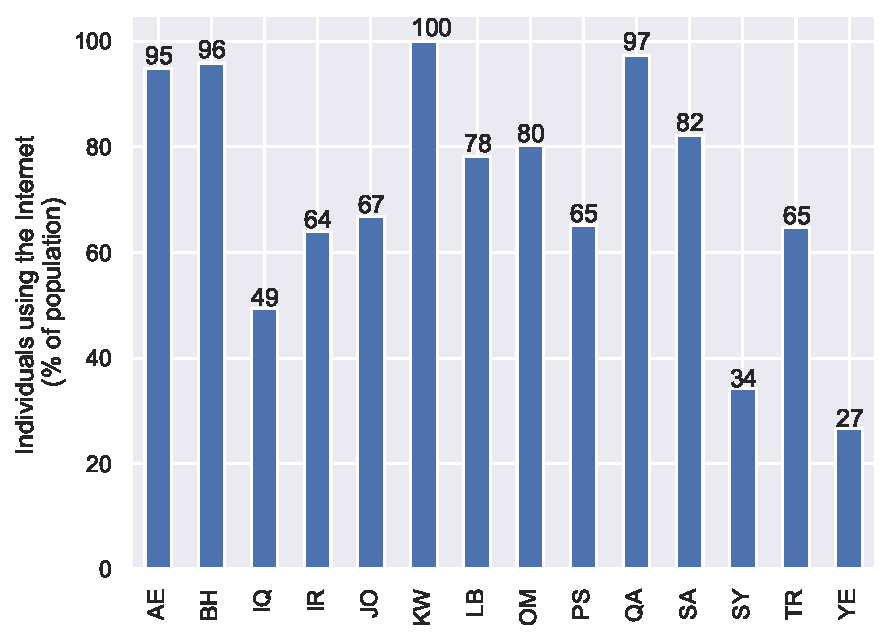
\includegraphics[width=0.75\linewidth]{../output/internet-users-2017.pdf}
    \caption{Percentage of population using the Internet in the Middle East in 2017}
    \label{fig:perc-internet-users-2017}
\end{figure}

\begin{figure}
    \centering
    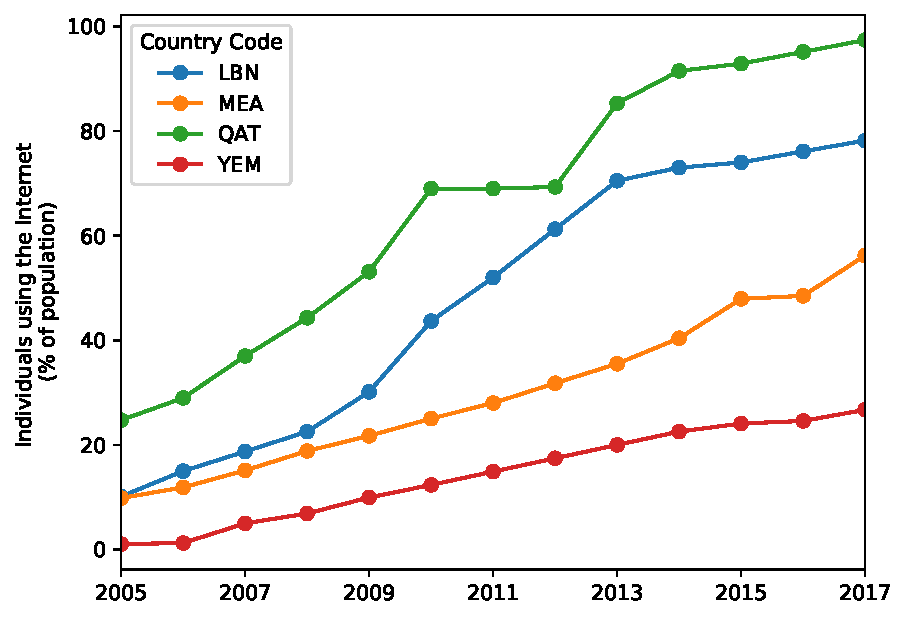
\includegraphics[width=0.75\linewidth]{../output/internet-users.pdf}
    \caption{Evolution of the percentage of population using the Internet for selected countries}
    \label{fig:perc-internet-users-evo}
\end{figure}

In order to get deeper insights on the evolution of the Internet penetration rate in Lebanon, we portray in Figure \ref{fig:population-internet-lb} the growth in the absolute number of users and the total population. In 2005, only 0.5 million individuals were using the Internet.

The population increase between 2011 and 2015 is mainly due to the Syrian refugees.   

\begin{figure}[!h]
    \centering
    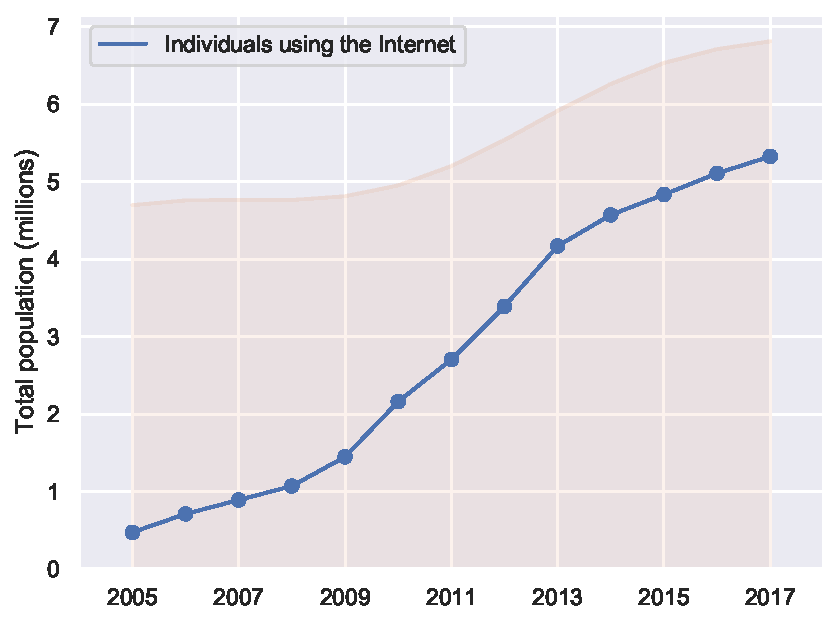
\includegraphics[width=0.75\linewidth]{../output/population-internet-lbn.pdf}
    \caption{Growth in the number of Internet users in Lebanon (indicated by dotted lines) and growth in population (indicated by shaded areas)}
    \label{fig:population-internet-lb}
\end{figure}

\begin{figure}
    \centering
    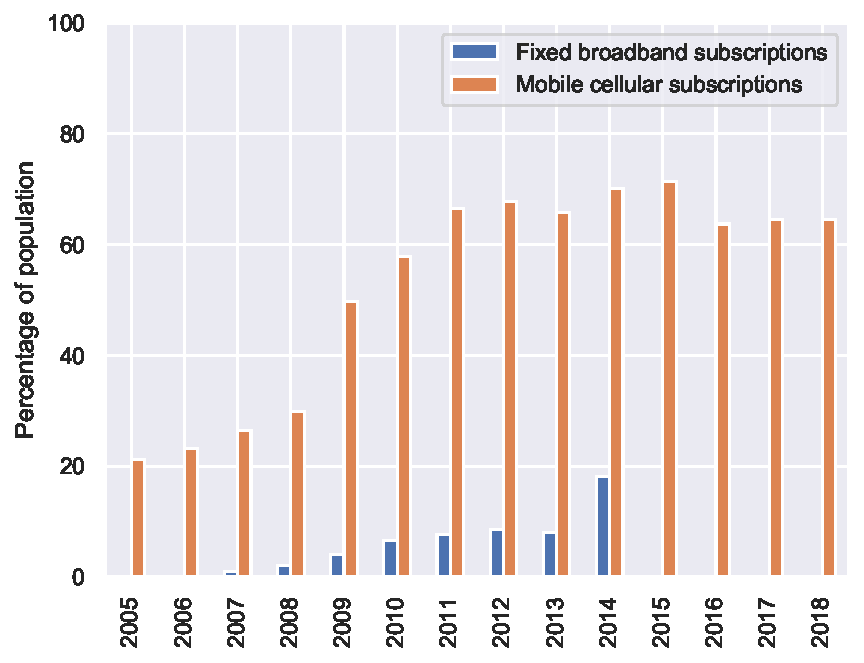
\includegraphics[width=0.75\linewidth]{../output/aggregate-lbs-users.pdf}
    \caption{test}
\end{figure}

\begin{figure}
    \centering
    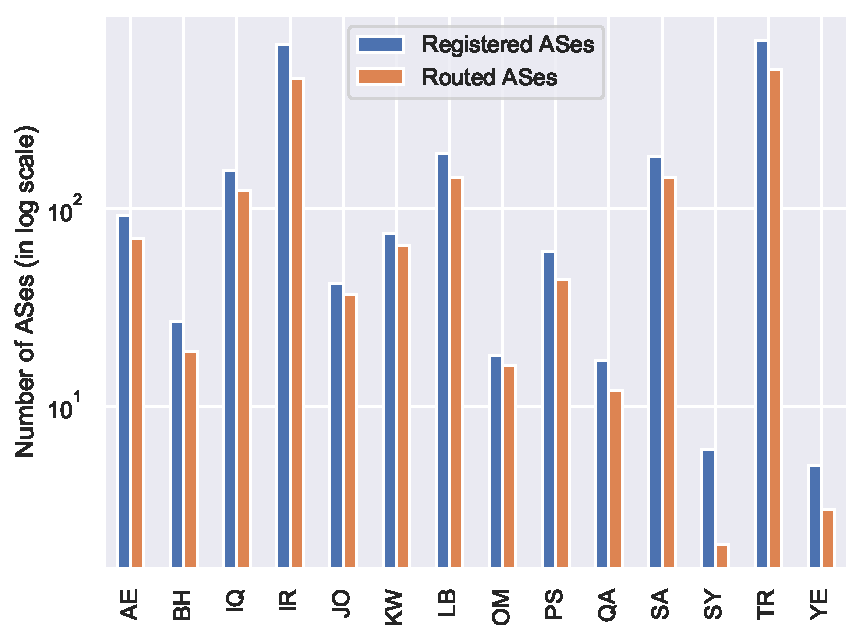
\includegraphics[width=0.75\linewidth]{../output/as-stat.pdf}
    \caption{test}
\end{figure}

% \begin{figure}
%     \centering
%     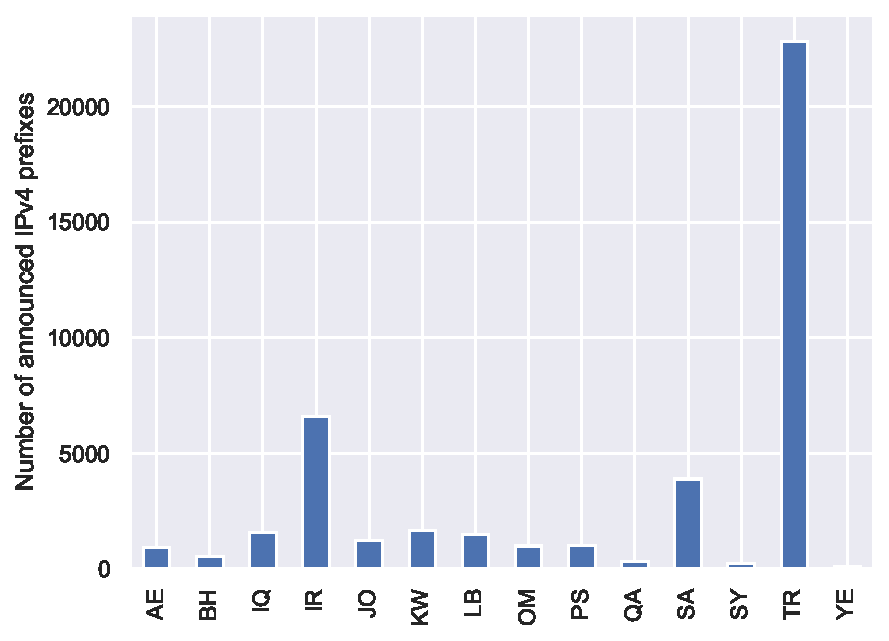
\includegraphics[width=0.75\linewidth]{../output/prefix-v4.pdf}
%     \caption{test}
% \end{figure}

% \begin{figure}
%     \centering
%     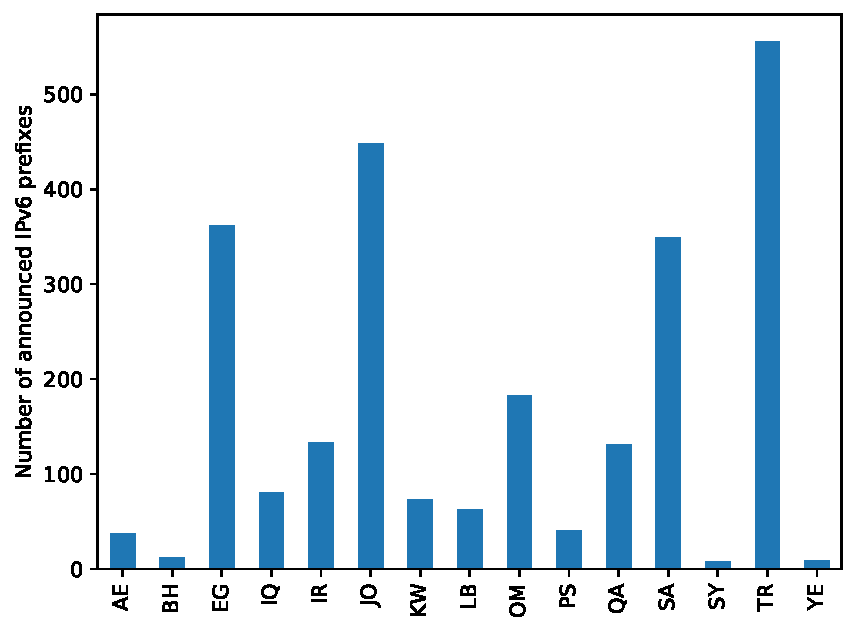
\includegraphics[width=0.75\linewidth]{../output/prefix-v6.pdf}
%     \caption{test}
% \end{figure}

\begin{figure}
    \centering
    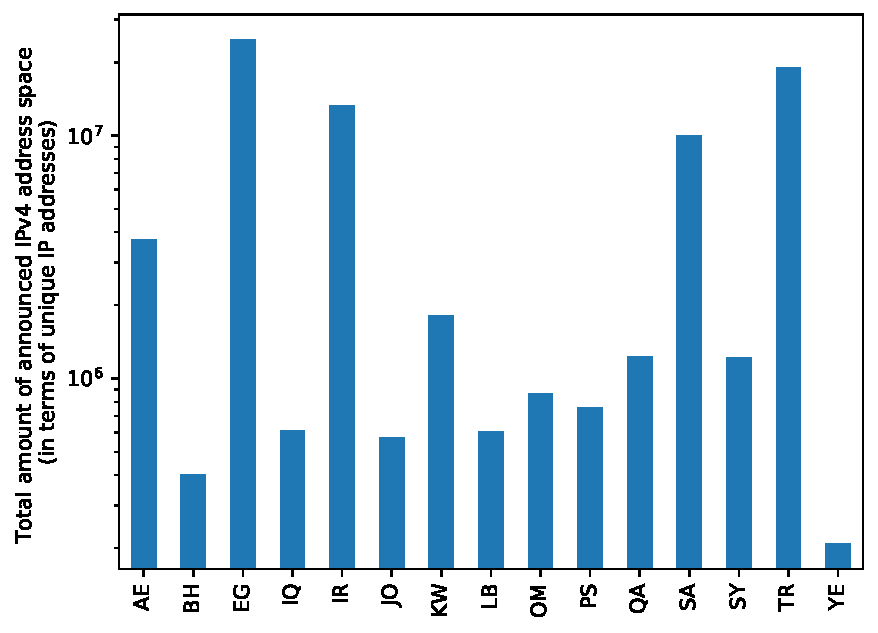
\includegraphics[width=0.75\linewidth]{../output/ips-v4.pdf}
    \caption{test}
\end{figure}

\begin{figure}
    \centering
    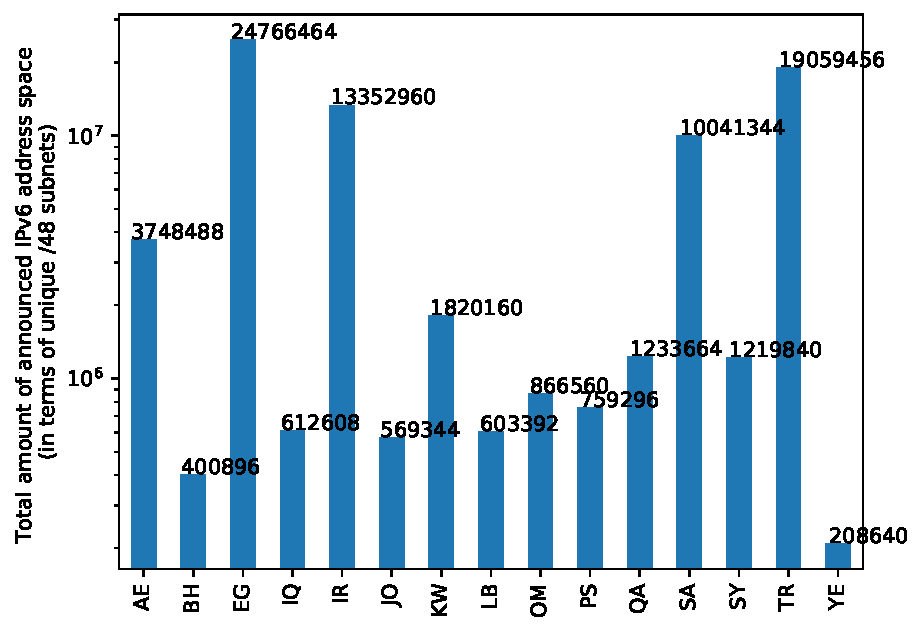
\includegraphics[width=0.75\linewidth]{../output/48s-v6.pdf}
    \caption{test}
\end{figure}

\begin{figure}
    \centering
    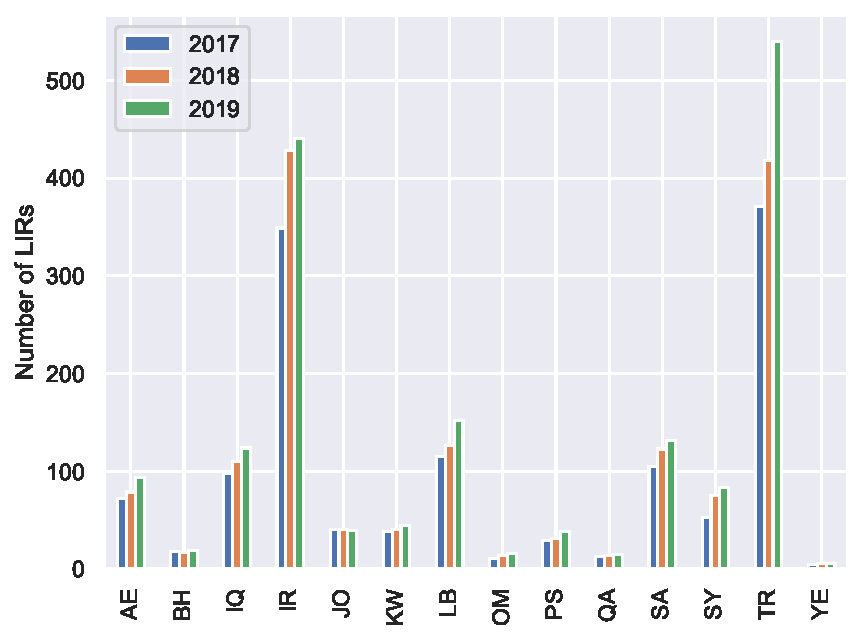
\includegraphics[width=0.75\linewidth]{../output/lir.pdf}
    \caption{test}
\end{figure}

\begin{figure}
    \centering
    \subcaptionbox{Frequency bands.\label{fig:perc-band-evo}}
    {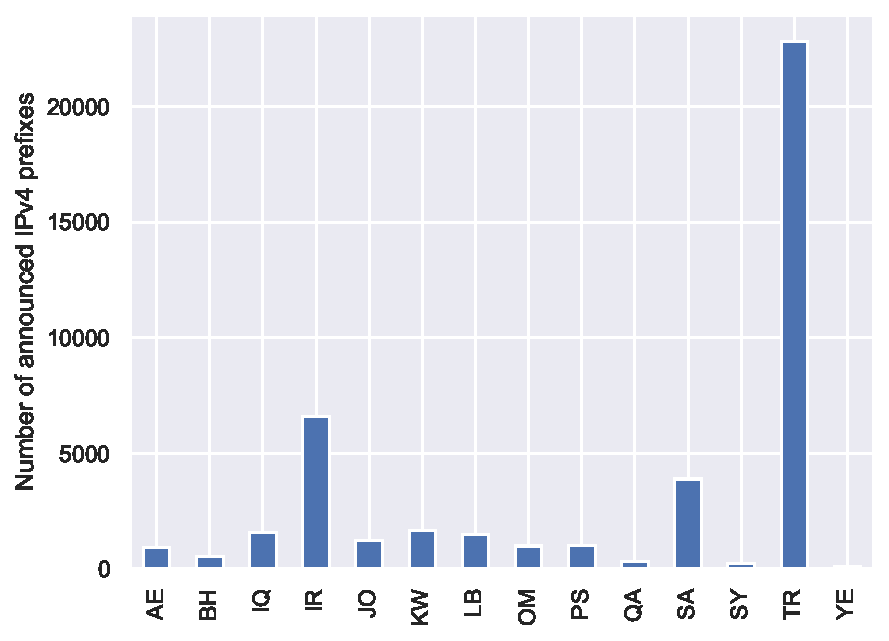
\includegraphics[width=0.45\linewidth]{../output/prefix-v4.pdf}}
    \subcaptionbox{Mobile technologies.\label{fig:perc-techno-evo}}
    {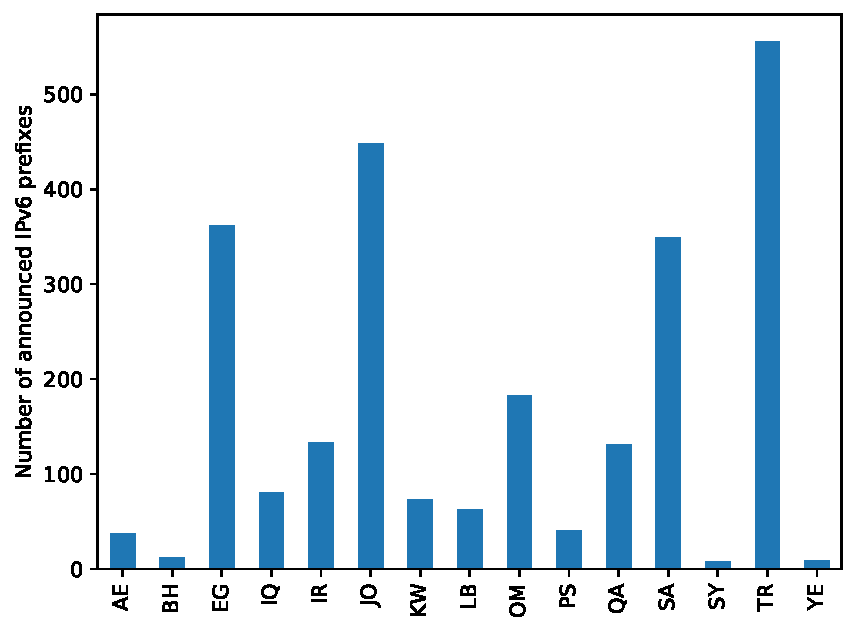
\includegraphics[width=0.45\linewidth]{../output/prefix-v6.pdf}}
    \caption{Evolution of the spectrum utilization in the city of Rennes in France.
    \label{fig:perc-antenna-evo}
    }
\end{figure}

\end{document}